\pagebreak
\subsection{Thermal Design} \label{Thermal_section}

\begin{centering}
The experiment will experience a wide range of temperatures during the flight and it must be able to continue to operate despite these changes. As seen in Figure \ref{fig:temperature-profile} the coldest point of the flight will be between 15km and 20km where the air temperature can drop to $-80\degree$C and temperatures on the gondola have been recorded as low as $-40\degree$C during the float phase in the past \cite{BexusManual}. In addition launching from Kiruna in late October means the temperature on the ground could be as low as $-15\degree$C. As our lowest operating temperature component must be at a minimum of $0\degree$C this could mean heaters may need to be switched on while the experiment is still on the ground. 
\end{centering}


\begin{figure}[H]
    \begin{align*}
        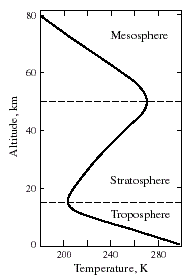
\includegraphics[height=5cm]{4-experiment-design/img/temperature-profile.png}
    \end{align*}
    \caption{Diagram showing the temperature profile of the atmosphere \cite{jacob}}\label{fig:temperature-profile}
\end{figure}


\begin{centering}
To protect the components against the cold two heaters will be included. One of these will be placed close to the Arduino, which is anticipated to be able to keep the controller area warm enough, and the second will be placed close to the valves to ensure they continue to operate as expected. To control these heaters two temperature sensors will also be onboard in similar locations. If the reading from one of the temperature sensors is lower than the predefined value then the heater will turn on. The predefined value will be chosen based upon the minimum operating temperature of the components. It is also expected that the electrical components will produce some heat themselves.
\end{centering}


\begin{centering}
In addition to using electrical heaters the experiment will also be thermally insulated. The Styrofoam casing which will be used to protect the CAC from impact forces will also serve as insulation. It is also planned to add additional insulation around the components.  
\end{centering}

\begin{centering}
It is also important to consider heating from the sun which could raise the temperature of the experiment considerably. Sufficient insulation should be included to ensure the inside of the box stays within the operating temperature range. This will be investigated at a later date when a full CFD thermal analysis is completed.
\end{centering}
\bigskip

\pagebreak


%Added this space to help us see all of the numbers. This "Track changes" sign blocks them every time!


\begin{longtable}{|m{1cm}|m{3.5cm}|m{1.3cm}|m{1.3cm}|m{1.4cm}|m{1.3cm}|m{1.3cm}|m{1.3cm}|}
\hline
\multirow{2}{*}{\textbf{ID}} & \multirow{2}{*}{\textbf{Components}}                                 & \multicolumn{2}{l|}{\textbf{Operating (°C)}} & \multicolumn{2}{l|}{\textbf{Survivable (°C)}} & \multicolumn{2}{l|}{\textbf{Expected (°C)}} \\ \cline{3-8} &   & Min.  & Max.  & Min.  & Max.  &  Min.   &  Max.            \\ \hline
E1 & Arduino Due & -40 & 85 & -60 & 150 & -30.62 & 24.01 \\ \hline
E2 & Ethernet Shield & -40 & 85 & -65 & 150 & -30.62 & 24.01 \\ \hline
E3 & Miniature diaphragm air pump & 5 & 40 & -10 & 40 & 10 & 34.93 \\ \hline
E4 & Pressure Sensor & -40 & 85 & -40 & 125 & -19.70 & 34.93 \\ \hline
E5 & Sampling Valve (inlet and outlet 1/8"" female) & -20 & 50 & -20\footnote{If survivable temperatures were not given, operating temperatures were used as survivable limits.\label{fn:erik}} & 50\textsuperscript{\ref{fn:erik}} & -15 & 20 \\ \hline
E6 & Airflow sensor AWM43300V & -20 & 70 & -20\textsuperscript{\ref{fn:erik}} & 70\textsuperscript{\ref{fn:erik}} & -8.77 & 34.93 \\ \hline
E7 & Heater ($12.7\times 50.8 mm$) & -200 & 200 & -200\textsuperscript{\ref{fn:erik}} & 200\textsuperscript{\ref{fn:erik}} & -20 & 36 \\ \hline
E8 & Voltage Regulator & -40 & 125 & -40\textsuperscript{\ref{fn:erik}} & 125\textsuperscript{\ref{fn:erik}} & -30.62 & 34.93 \\ \hline
E9 & Temperature Sensor & -55 & 125 & -65 & 150 & -19.70 & 34.93 \\ \hline
E10 & DCDC 24 V & -40 & 85 & -55 & 125 & -19.70 & 34.93 \\ \hline
E12 & Micro SD & -25 & 85 & -200\textsuperscript{\ref{fn:erik}} & 200\textsuperscript{\ref{fn:erik}} & -19.70 & 34.93 \\ \hline
% E13 & Logic CAT5E & -20 & 75 & (-20)\textsuperscript{\ref{fn:erik}} & (75)\textsuperscript{\ref{fn:erik}} & TBD\textsuperscript{\ref{fn:ivan}} & TBD\textsuperscript{\ref{fn:ivan}} \\ \hline
% E14 & Resistors (33, 150 and 100 ohm) & -55 & 155 & (-55)\textsuperscript{\ref{fn:erik}} & (155)\textsuperscript{\ref{fn:erik}} & TBD\textsuperscript{\ref{fn:ivan}} & TBD\textsuperscript{\ref{fn:ivan}} \\ \hline
% E15 & Capacitors $(0.1 \mu$ F and $10 \mu$ F) & -30 & 85 & (-200)\textsuperscript{\ref{fn:erik}} & (200)\textsuperscript{\ref{fn:erik}} & TBD\textsuperscript{\ref{fn:ivan}} & TBD\textsuperscript{\ref{fn:ivan}} \\ \hline
E16 & Mosfet for current control & -55 & 175 & -55 & 175 & -20 & -20 \\ \hline
E17 & Diodes for DCDC converters & -65 & 175 & -65\textsuperscript{\ref{fn:erik}} & 175\textsuperscript{\ref{fn:erik}} & -19.70 & 34.93 \\ \hline
E18 & 3.3V LED & -40 & 85 & -40\textsuperscript{\ref{fn:erik}} & 85\textsuperscript{\ref{fn:erik}} & -19.70 & 24.01 \\ \hline 
E19 & 15-pin D-SUB Female connector with pins & -55 & 120 & -200\textsuperscript{\ref{fn:erik}} & 200\textsuperscript{\ref{fn:erik}} & -8.77 & 24.01 \\ \hline
E20 & 9-pin D-SUB Female connector with pins & -55 & 120  & -200\textsuperscript{\ref{fn:erik}} & 200\textsuperscript{\ref{fn:erik}} & -8.77 & 24.01 \\ \hline
E21 & 9-pin D-SUB Female connector with soldering cups & -55 & 105 & -55\textsuperscript{\ref{fn:erik}} & 105\textsuperscript{\ref{fn:erik}} & -8.77 & 24.01 \\ \hline
E22 & 9-pin D-SUB Male connector with soldering cups & -55 & 105 & -55\textsuperscript{\ref{fn:erik}} & 105\textsuperscript{\ref{fn:erik}} & -8.77 & 24.01 \\ \hline
E23 & 15-pin D-SUB Male connector with soldering cups & -55  & 105 & -55\textsuperscript{\ref{fn:erik}} & 105\textsuperscript{\ref{fn:erik}} & -8.77 & 24.01 \\ \hline
E24 & 9-pin D-SUB backing & -40 & 120 & -40\textsuperscript{\ref{fn:erik}} & 120 & -8.77 & 24.01  \\ \hline
E25 & 15-pin D-SUB backing & -40 & 120 & -40\textsuperscript{\ref{fn:erik}} & 120 & -8.77 & 24.01  \\ \hline
% E26 & Wall mounting bolts & TBD\textsuperscript{\ref{fn:ivan}} & TBD\textsuperscript{\ref{fn:ivan}} & TBD\textsuperscript{\ref{fn:ivan}} & TBD\textsuperscript{\ref{fn:ivan}} & TBD\textsuperscript{\ref{fn:ivan}} & TBD\textsuperscript{\ref{fn:ivan}} \\ \hline
E27 & D-SUB cable CAC to AAC & -40 & 85 & -55 & 125 & -40 & 40 \\ \hline
% E28 & 3.3 Zener diode & TBD\textsuperscript{\ref{fn:ivan}} & 175 & TBD\textsuperscript{\ref{fn:ivan}} & (175)\textsuperscript{\ref{fn:erik}} & TBD\textsuperscript{\ref{fn:ivan}} & TBD\textsuperscript{\ref{fn:ivan}} \\ \hline
E29 & Male connector on PCB & -40 & 85 & -40\textsuperscript{\ref{fn:erik}} & 85 & -8.77 & 24.01 \\ \hline
E30 & Female connector from wall & -40 & 85 & -40\textsuperscript{\ref{fn:erik}} & 85 & - & - \\ \hline
% E31 & Grounding contact & -55 & 125 & (-55)\textsuperscript{\ref{fn:erik}} & (125)\textsuperscript{\ref{fn:erik}} & TBD\textsuperscript{\ref{fn:ivan}} & TBD\textsuperscript{\ref{fn:ivan}} \\ \hline
E32 & Logic CAT5 E-link for inside box &-20 & 75 & -20\textsuperscript{\ref{fn:erik}} & 75\textsuperscript{\ref{fn:erik}} & -15 & 20 \\ \hline
E33 & Signal Wires & -60 & 200 & -60\textsuperscript{\ref{fn:erik}} & 200\textsuperscript{\ref{fn:erik}} & - & - \\ \hline
E34 & Flushing valve (inlet and outlet 1/8"" female) & -10 & 50 & -10\textsuperscript{\ref{fn:erik}} & 50\textsuperscript{\ref{fn:erik}} & -7.36 & 42.53 \\ \hline
E35 & Valves manifold (outlet 1/8"" female) & -10 & 50 & -10\textsuperscript{\ref{fn:erik}} & 50\textsuperscript{\ref{fn:erik}} & -6.77 & 40.504 \\ \hline
E36 & Power wire black & -60 & 200 & -60\textsuperscript{\ref{fn:erik}} & 200\textsuperscript{\ref{fn:erik}} & - & - \\ \hline
% E37 & Electrical Tape for marking wires (White) & -10 & 90 & (-10)\textsuperscript{\ref{fn:erik}} & (90)\textsuperscript{\ref{fn:erik}} & TBD\textsuperscript{\ref{fn:ivan}} & TBD\textsuperscript{\ref{fn:ivan}} \\ \hline
% E38 & Electrical Tape for marking wires (Black) & -10 & 90 & (-10)\textsuperscript{\ref{fn:erik}} & (90)\textsuperscript{\ref{fn:erik}} & TBD\textsuperscript{\ref{fn:ivan}} & TBD\textsuperscript{\ref{fn:ivan}} \\ \hline
% E39 & Electrical Tape for marking wires (Green) & -10 & 90 & (-10)\textsuperscript{\ref{fn:erik}} & (90)\textsuperscript{\ref{fn:erik}} & TBD\textsuperscript{\ref{fn:ivan}} & TBD\textsuperscript{\ref{fn:ivan}} \\ \hline
% E40 & Electrical Tape for marking wires (Violet) & -10 & 90 & (-10)\textsuperscript{\ref{fn:erik}} & (90)\textsuperscript{\ref{fn:erik}} & TBD\textsuperscript{\ref{fn:ivan}} & TBD\textsuperscript{\ref{fn:ivan}} \\ \hline
% E41 & Electrical Tape for marking wires (Gray) & -10 & 90 & (-10)\textsuperscript{\ref{fn:erik}} & (90)\textsuperscript{\ref{fn:erik}} & TBD\textsuperscript{\ref{fn:ivan}} & TBD\textsuperscript{\ref{fn:ivan}} \\ \hline
% E42 & Electrical Tape for marking wires (Brown) & -10 & 90 & (-10)\textsuperscript{\ref{fn:erik}} & (90)\textsuperscript{\ref{fn:erik}} & TBD\textsuperscript{\ref{fn:ivan}} & TBD\textsuperscript{\ref{fn:ivan}} \\ \hline
% E43 & Electrical Tape for marking wires (Blue) & -10 & 90 & (-10)\textsuperscript{\ref{fn:erik}} & (90)\textsuperscript{\ref{fn:erik}} & TBD\textsuperscript{\ref{fn:ivan}} & TBD\textsuperscript{\ref{fn:ivan}} \\ \hline
% E44 & Heat shrinking tube 2.5 x 1mm & -55 & 125 & (-55)\textsuperscript{\ref{fn:erik}} & (125)\textsuperscript{\ref{fn:erik}} & TBD\textsuperscript{\ref{fn:ivan}} & TBD\textsuperscript{\ref{fn:ivan}} \\ \hline
E45 & 25-pin D-SUB female connector with pins & -10 & 90 & -10\textsuperscript{\ref{fn:erik}} & 90\textsuperscript{\ref{fn:erik}} & -8.77 & 24.01 \\ \hline
E46 & 25-pin D-SUB male connector with soldering cups & -10 & 90 & -10\textsuperscript{\ref{fn:erik}} & 90\textsuperscript{\ref{fn:erik}} & -8.77 & 24.01 \\ \hline
E47 & 25-pin D-SUB backing & -10 & 90 & -10\textsuperscript{\ref{fn:erik}} & 90\textsuperscript{\ref{fn:erik}} & -8.77 & 24.01 \\ \hline
E48 & Power wire red & -60 & 200 & -60\textsuperscript{\ref{fn:erik}} & 200
\textsuperscript{\ref{fn:erik}} & - & -  \\ \hline
% E49 & Potentiometer 1k ohm & -55 & 125 & (-55)\textsuperscript{\ref{fn:erik}} & (120)\textsuperscript{\ref{fn:erik}} & TBD\textsuperscript{\ref{fn:ivan}} & TBD\textsuperscript{\ref{fn:ivan}} \\ \hline
E50 & 6-pin male & -55 & 105 & -55\textsuperscript{\ref{fn:erik}} & 105\textsuperscript{\ref{fn:erik}} & -8.77 & 24.01  \\ \hline
E51 & 8-pin male single row header& -40 & 105 & -40\textsuperscript{\ref{fn:erik}} & 105\textsuperscript{\ref{fn:erik}} & -8.77 & 24.01  \\ \hline
E52 & 10-pin male single row header & -55 & 105 & -55\textsuperscript{\ref{fn:erik}} & 105\textsuperscript{\ref{fn:erik}} & -8.77 & 24.01  \\ \hline
E53 & 36-pin male double row header & -40 & 105 & -40 & 125 & -8.77 & 24.01  \\ \hline
E54 & 12 V DC/DC converter & -40 & 85 & -55 & 125 & -8.77 & 24.01  \\ \hline
E56 & Pressure Sensor & -40 & 120 & -40\textsuperscript{\ref{fn:erik}} & 120\textsuperscript{\ref{fn:erik}} &  -8.77 & 34.93 \\ \hline


\caption{Table of Component Temperature Ranges.}
\label{tab:thermal-table}
\end{longtable}
\raggedbottom










\raggedbottom

\subsubsection{Internal Temperature}

As the current experiment model stands, an enclosed partition has been reserved in the lower front-right corner of the AAC section of the TUBULAR experiment. This partition will house all of the electronic components not required to be situated in specified locations throughout the experiment setting, as well as the pump and valves. The partition will occupy a space measuring 20 cm in length, 10 cm in width, and 20 cm in height, and will be insulated from inside to outside with polyethylene, polystyrene, and finally aluminum. The infrastructure within this enclosure shall be such that the electronics are fitted together to in turn be bound within another box of insulated material (likely made from PVC) and will be appropriately labeled the "Electronics Box." Subsequently, above the electronics box will be situated the pump and the collection of valves - the valves being routed together by several tubes to form a compact structure with the label "Valve Center" ascribed to it. As previously mentioned regarding the heaters, one will be included in the electronics box with its main priority being keeping the Arduino Due board within operational temperatures, and delivering the remaining heat to peripheral electronics. The other heater will be fitted between the diaphragm of the pump and the entrances to the valve center and will carry the task of keeping its lateral neighbors within their respective functional temperature ranges.

The pump has the most critical temperature range in that it is the only component that cannot operate below freezing temperatures - in fact, it must always be no colder than $5\degree$C, or the EPDM diaphragm will not be able to expand and contract sufficiently to maintain the desired airflow of 8L/min. The valves are also crucial to the experiment's function, as their correct function is what enables each and every sampling bag onboard to be used. For this reason, while the valves can operate down to $-43\degree$C, they still need to be kept above this limit whenever in use.

Given the thermal conductivity of EPDM ($0.2 W/(m.K)$), the diaphragm experiences a minimal temperature drop across itself when one side is subject to the heater's temperature while the other end of the pump is leveled with the ambient temperature. Case in point, it was found that at an ambient temperature of $-50\degree$C and a heater temperature at $10\degree$C, that the center of the pump - the far end of the diaphragm - measured $9.35\degree$C. Reassessing the equation yielded the most energy-conserving temperature that would keep the pump's diaphragm above the minimum requirement to be $7\degree$C - and this held whether the temperature were as it could be on ground level ($-10\degree$C), or in floating phase ($-50\degree$C).



\subsubsection{Box Analysis}